\documentclass[aspectratio=169,spanish]{beamer}
\usepackage[utf8]{inputenc}
\usepackage{amsmath}
\usepackage{bm}
\usefonttheme{professionalfonts}
\title{Estadística III}
\subtitle{Splines}
\author{Alejandro López Hernández}
\institute{FES Acatlán - UNAM}
\date{\today}
\usetheme{Pittsburgh}
\usecolortheme{beaver}

\begin{document}

\frame{\titlepage}

\begin{frame}
\frametitle{Índice}
\tableofcontents
\end{frame}

\begin{frame}
\frametitle{Introducción}
\section{Introducción}
Derivado de los métodos lineales de regresión nos enfocaremos en un método llamado \textbf{Splines Penalizados}, la idea es utilizar una base de funciones con las que podamos generar funciones continuas que suavicen nuestros datos. 
\end{frame}

\begin{frame}
\frametitle{1-Spline}
\section{1-Spline}
La idea principal es poder ajustar datos con estructuras no lineales, si suponemos un modelo $y_i=\beta_0+\beta_1x_i+\varepsilon_i$ estamos limitados a solo ajustar datos lineales, con este modelo nuestra base de funciones es $\{1,x\}$, lo que se propone hacer con los 1-splines es dividir el rango la regresión en varios intervalos que de forma local si tengan un comportamiento lineal. 
\end{frame}


\begin{frame}
\frametitle{1-Spline}
\center
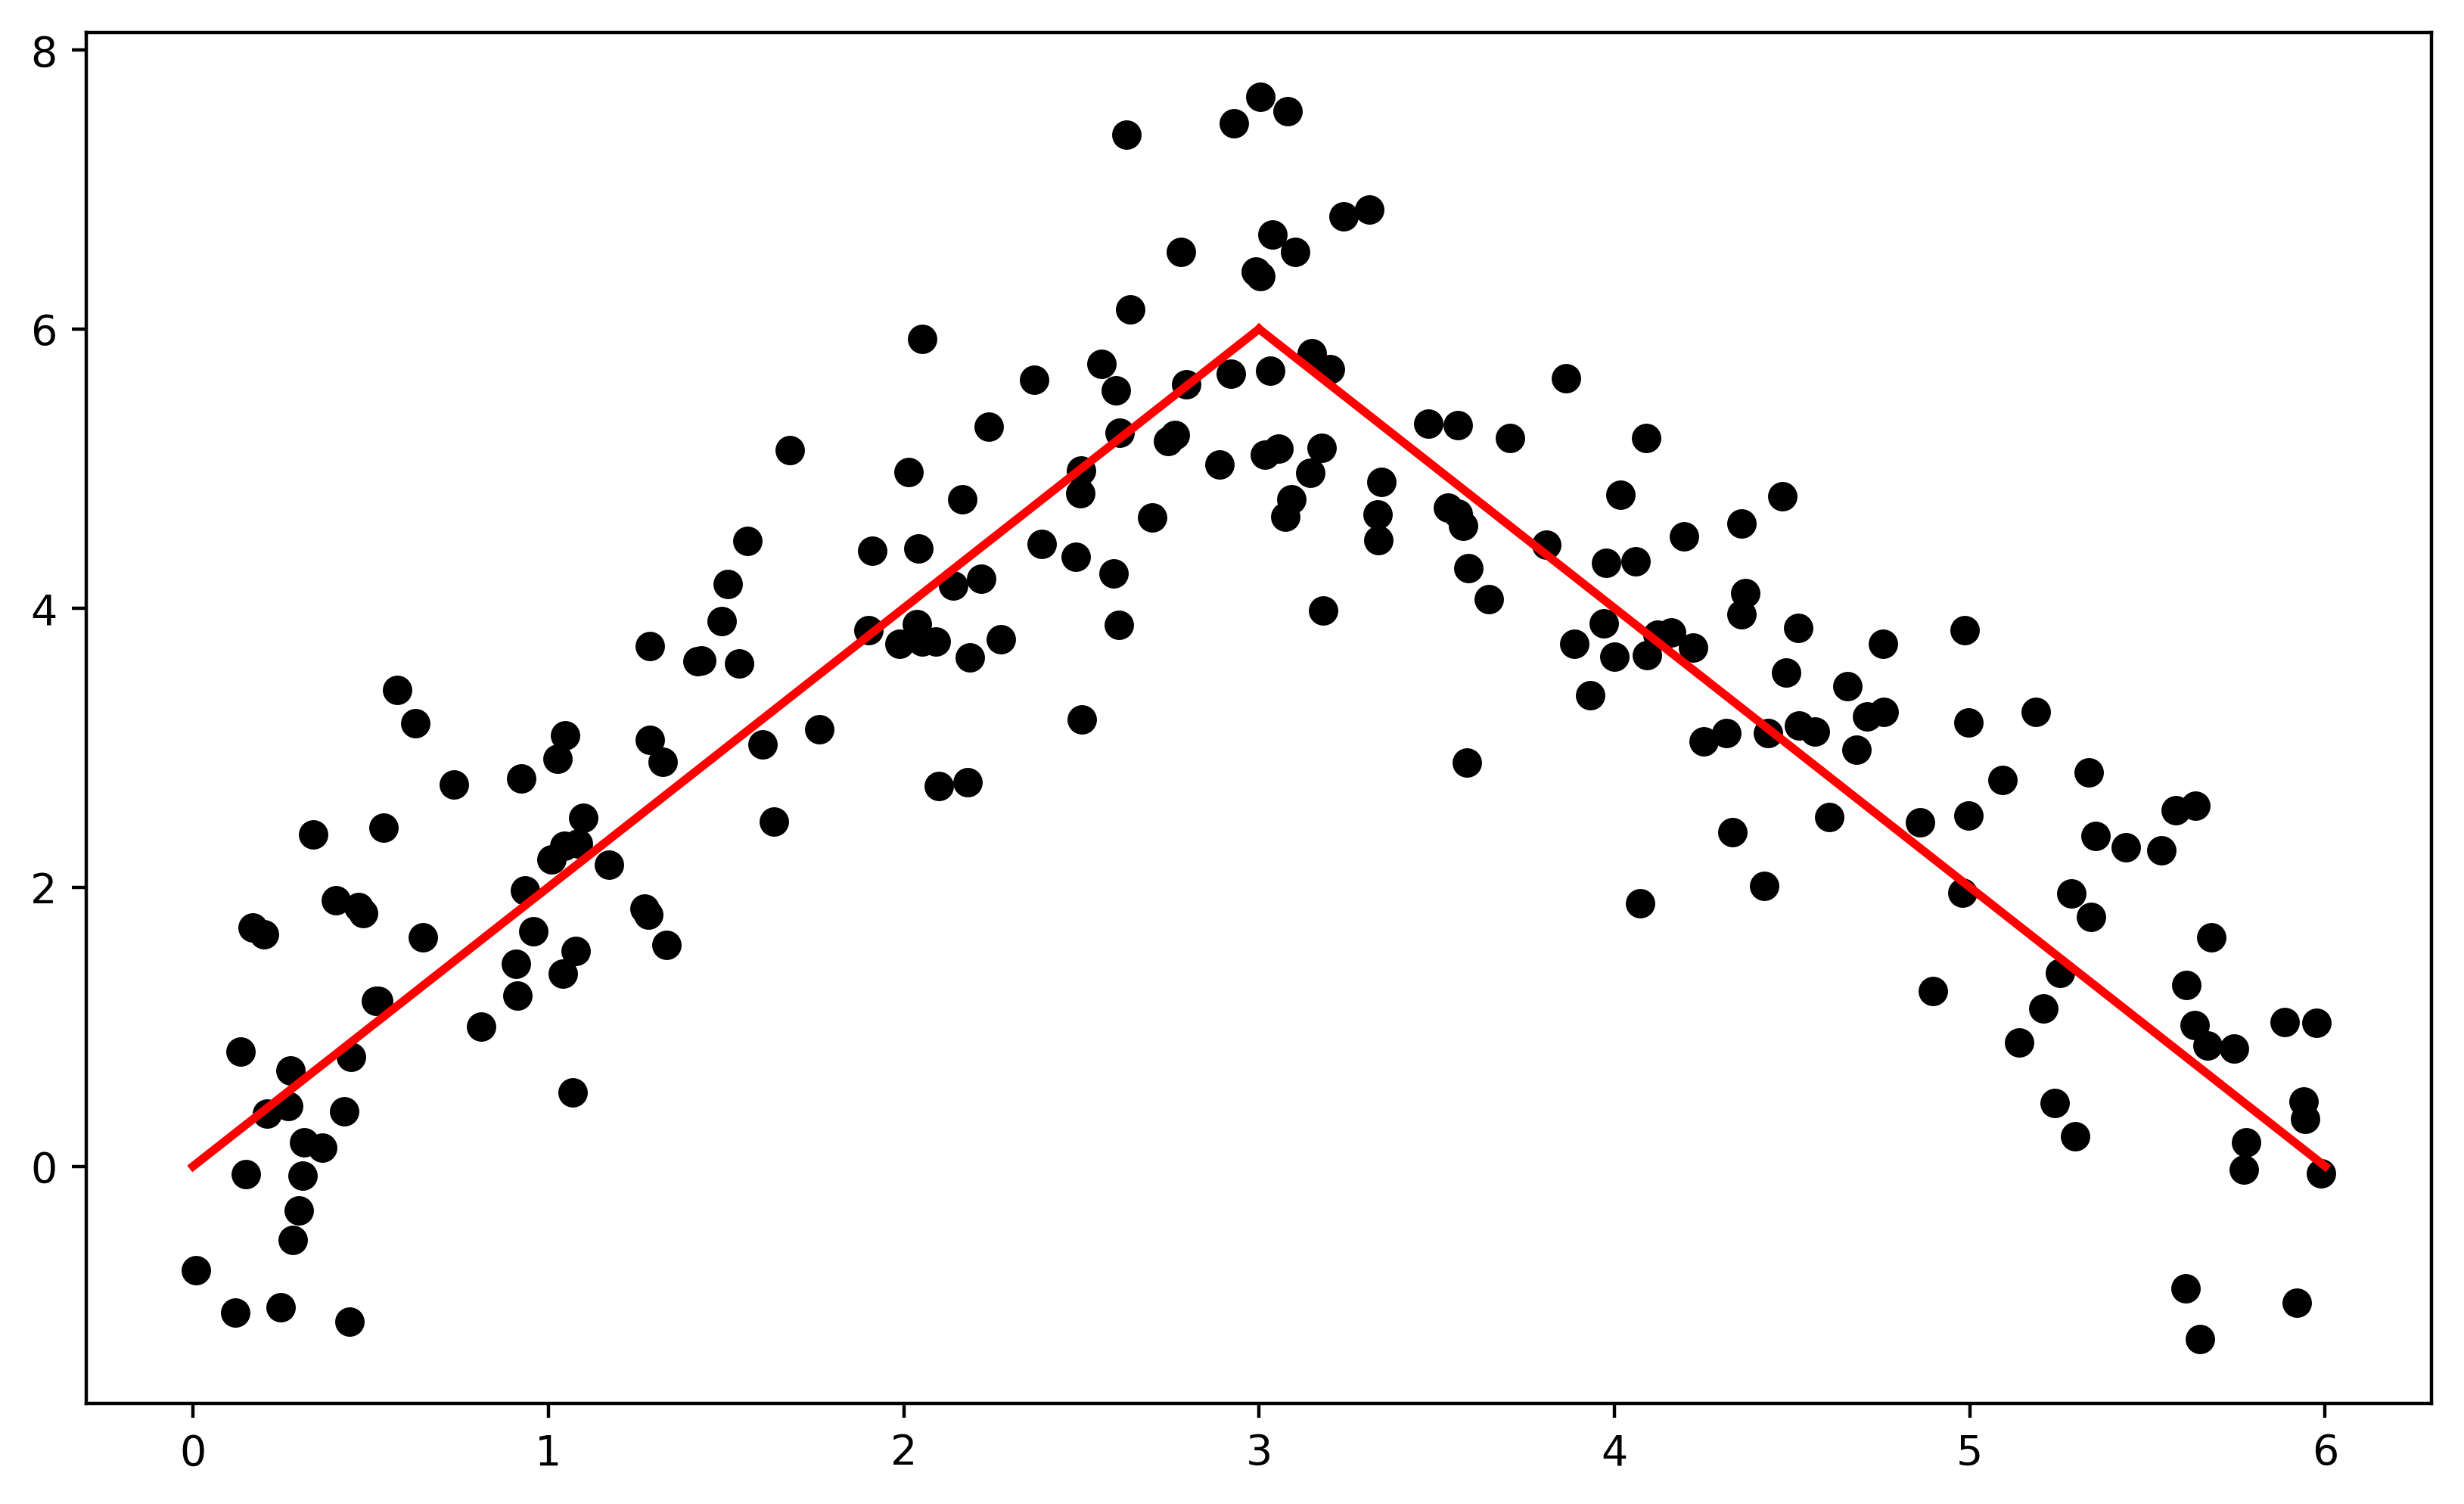
\includegraphics[scale=0.5]{spline1}
\end{frame}


\begin{frame}
\frametitle{1-Spline}
En este caso la regresión la obtuvimos con $$f(x) = 0 + 2x - 4 (x-3)_{+}$$
donde $u_{+}=\max\{u,0\}$, de esta forma estamos extendiendo la base a $\{1,x,(x-3)_{+}\}$, y nos da la facilidad de ajustarnos a estructuras mas complejas. 
En general, podemos hacer tantos cortes como deseamos, estos cortes son llamados \textbf{nudos}, si decidimos realizar $K$ nudos nuestra base sera $\{1,x,(x-\kappa_1)_{+},(x-\kappa_2)_{+},...,(x-\kappa_K)_{+}\}$, por lo tanto hay que estimar $K+2$ parámetros $\beta_0,\beta_1,b_1,...,b_{K}$, y nuestra regresión es. $$ f(x) = \beta_0+\beta_1 x + \sum_{k=1}^{K}b_k (x-\kappa_k)_{+}$$
\end{frame}


\begin{frame}
\frametitle{1-Spline}
Para expresar nuestro problema de forma lineal podemos escribir 
\begin{equation*}
\bm{X} = 
\begin{bmatrix}
1 & x_1 & (x_1-\kappa_1)_{+} & \cdots &(x_1-\kappa_K)_{+}\\
\vdots & \vdots & \vdots & \ddots &\vdots\\
1 & x_n & (x_n-\kappa_1)_{+} & \cdots &(x_n-\kappa_K)_{+}
\end{bmatrix}
\end{equation*}
\begin{equation*}
\bm{\beta} = 
\begin{bmatrix}
\beta_0 & \beta_1 & b_1 & \cdots & b_K
\end{bmatrix}^T
\end{equation*}
\begin{equation*}
\bm{y} = 
\begin{bmatrix}
y_1 & y_2 & y_3 & \cdots & y_n
\end{bmatrix}^T
\end{equation*}
Por lo tanto nuestro problema se reduce a minimizar $$\| \bm{y} - \bm{X\beta}\|^2$$
\end{frame}

\begin{frame}
\frametitle{1-Spline}
Sin embargo, hay que restringir los coeficientes de los nudos con el objetivo de tener un control sobre la suavidad de la regresión. Esta restricción se solucionando agregando la restricción $\bm{\beta}^T\bm{D}\bm{\beta}\le C$ donde:
\begin{equation*}
\bm{D} = 
\begin{bmatrix}
0&0&0&0&0&\cdots&0\\
0&0&0&0&0&\cdots&0\\
0&0&1&0&0&\cdots&0\\
0&0&0&1&0&\cdots&0\\
\vdots&\vdots&\vdots&\vdots&\vdots&\ddots&\vdots\\
0&0&0&0&0&\cdots&1
\end{bmatrix} = 
\begin{bmatrix}
\bm{0}_{2\times 2}&\bm{0}_{2\times K}\\
\bm{0}_{K\times 2}&\bm{I}_{K\times K}
\end{bmatrix}=\text{diag}(0,0,1,..,1)
\end{equation*}

de esta manera nuestro problema se puede resolver utilizando un multiplicador de Lagrange:
$$\text{mínimizar } \| \bm{y} - \bm{X\beta}\|^2 + \lambda^2\bm{\beta}^T\bm{D}\bm{\beta}$$ para algún $\lambda>0$
\end{frame}

\begin{frame}
\frametitle{1-Spline}
Bueno, pues resulta que la solución es:
$$\hat{\bm{\beta}}_\lambda = (\bm{X}^T\bm{X}+\lambda^2\bm{D})^{-1}\bm{X}^T\bm{y} $$
\end{frame}



\begin{frame}
\frametitle{2-Spline}
\section{2-Spline}
De forma totalmente análoga que con los 1-Spline, la idea es ajustar curvas en ciertos intervalos, en este caso curvas cuadráticas. La ventaja de usar una curva cuadrática en lugar de lineales es que en los nudos tendremos funciones con derivadas (en lugar de picos). Nuestra base ahora será $\{1,x,x^2,(x-\kappa_1)^2_{+},(x-\kappa_2)^2_{+},...,(x-\kappa_K)^2_{+}\}$ y nuestra función tendrá que ajustar $K+3$ parámetros
$$ f(x) = \beta_0+\beta_1 x + \beta_2 x^2 +\sum_{k=1}^{K}b_k (x-\kappa_k)^2_{+}$$
\end{frame}


\begin{frame}
\frametitle{2-Spline}
El problema resulta el mismo 
$$\text{mínimizar } \| \bm{y} - \bm{X\beta}\|^2 + \lambda^2\bm{\beta}^T\bm{D}\bm{\beta}$$
pero con $\bm{D} = \text{diag}(0,0,0,1,..,1)$, y los parámetros extra a estimar. 
La solución resulta: 
$$\hat{\bm{\beta}}_\lambda = (\bm{X}^T\bm{X}+\lambda^4\bm{D})^{-1}\bm{X}^T\bm{y} $$
\end{frame}
\begin{frame}
\frametitle{p-Spline}
\section{p-Spline}
De forma mas general, se pueden definir bases que tengan derivadas de orden mas alto en los nudos. En general la base es de la forma $$\{1,x,x^2,...,x^p,(x-\kappa_1)^p_{+},(x-\kappa_2)^p_{+},...,(x-\kappa_K)^p_{+}\}$$
por lo tanto nuestra regresión es de la forma 
$$ f(x) = \beta_0+\beta_1 x + \beta_2 x^2 +...+\beta_p x^p+\sum_{k=1}^{K}b_k (x-\kappa_k)^p_{+}$$

\end{frame}

\begin{frame}
\frametitle{p-Spline}

El problema es totalmente análogo, solo que con más parámetros que estimar 
$$\text{mínimizar } \| \bm{y} - \bm{X\beta}\|^2 + \lambda^2\bm{\beta}^T\bm{D}\bm{\beta}$$
con $\bm{D} = \text{diag}(\bm{0}_{p+1},\bm{1}_{K})$
La solución resulta: 
$$\hat{\bm{\beta}}_\lambda = (\bm{X}^T\bm{X}+\lambda^{2p}\bm{D})^{-1}\bm{X}^T\bm{y} $$
\end{frame}

\end{document}